%\documentclass[a4paper]{leaflet}
%%\pdfpagewidth=420mm
%\pdfpageheight=\paperheight
%\usepackage{lipsum}
%%\usepackage{fontspec}
%\begin{document}
%%\title{GPG: A Guide by DUCS \Lclass{leaflet}}

%\title{The document class \Lclass{leaflet}}
%\author{%
 % Rolf Niepraschk\\
 % Walter Schmidt\\
 % Hubert G\"a\ss lein}
%\date{Last updated~\docdate\\printed \today}
%BLAH
%\end{document}

%%%%%%%%%%%%%%%%%%%%%%%%%%%%%%%%%%%%%%%%%%%%%%%%%%%%%%%%%%%%%%%%

%%
%% This is file `leaflet-manual.tex',
%% generated with the docstrip utility.
%%
%% The original source files were:
%%
%% leaflet.dtx  (with options: `manual')
%% 
%% Copyright (C) 2003, 2004
%% Rolf Niepraschk, Rolf.Niepraschk@ptb.de
%% Hubert Gaesslein, HubertJG@open.mind.de
%% 
%% This work may be distributed and/or modified under the
%% conditions of the LaTeX Project Public License, either version 1.3
%% of this license or (at your option) any later version.
%% The latest version of this license is in
%%   http://www.latex-project.org/lppl.txt
%% and version 1.3 or later is part of all distributions of LaTeX
%% version 2003/12/01 or later.
%% 
%% This work has the LPPL maintenance status "author-maintained".
%% 
\def\filename{leaflet-manual.tex}
\def\fileversion{v0.1}   % change this when leaflet-manual changed, too.
\def\filedate{2012/05/29}
\def\docdate {May 2012} % change this when leaflet-manual changed, too.
\listfiles
\errorcontextlines=99
\documentclass[
notumble, %% -- turns bottom page over for proofreading
%%nofoldmark,
%%dvipdfm,
%%portrait,
%%titlepage,
%%nocombine,
%%a3paper,
%%debug,
%%nospecialtricks,
%%draft,
]{leaflet}


\renewcommand*\foldmarkrule{.3mm}
\renewcommand*\foldmarklength{5mm}

\usepackage[T1]{fontenc}
\usepackage{textcomp}
\usepackage{mathptmx}
\usepackage[scaled=0.9]{helvet}
\makeatletter
\def\ptmTeX{T\kern-.1667em\lower.5ex\hbox{E}\kern-.075emX\@}
\DeclareRobustCommand{\ptmLaTeX}{L\kern-.3em
        {\setbox0\hbox{T}%
         %\vb@xt@ % :-)
         \vbox to\ht0{\hbox{%
                            \csname S@\f@size\endcsname
                            \fontsize\sf@size\z@
                            \math@fontsfalse\selectfont
                            A}%
                      \vss}%
        }%
        \kern-.12em
        \ptmTeX}
\makeatother
\let\TeX=\ptmTeX
\let\LaTeX=\ptmLaTeX
\usepackage{shortvrb}
\MakeShortVerb{\|}
\usepackage{url}
\usepackage{graphicx}
\usepackage[dvipsnames,usenames]{color}
\definecolor{LIGHTGRAY}{gray}{.9}

%%%%\renewcommand{\descfont}{\normalfont}
\newcommand\Lpack[1]{\textsf{#1}}
\newcommand\Lclass[1]{\textsf{#1}}
\newcommand\Lopt[1]{\texttt{#1}}
\newcommand\Lprog[1]{\textit{#1}}

\newcommand*\defaultmarker{\textsuperscript\textasteriskcentered}

\title{\textit{GNU Privacy Guard}: \\A CompSoc guide to daily use of email encryption\\\vskip1.5em Mac Edition}
\author{%
  Martin Dehnel\\
  James Fielder\\ 
  (Durham University)
  }
\date{~\docdate}% \vskip11em}

%\CutLine*{1}% Dotted line without scissors
%\CutLine{6}%  Dotted line with scissors

%\AddToBackground{5}{%  Background of a small page
%  \put(0,0){\textcolor{Cerulean}{\rule{\paperwidth}{\paperheight}}}}

%\AddToBackground*{2}{% Background of a large page
%  \put(\LenToUnit{.5\paperwidth},\LenToUnit{.5\paperheight}){%
%    \makebox(0,0)[c]{%
%      \resizebox{.9\paperwidth}{!}{\rotatebox{35.26}{%
%        \textsf{\textbf{\textcolor{LIGHTGRAY}{BACKGROUND}}}}}}}}

\begin{document}
\maketitle

\includegraphics[width=0.9\paperwidth]{images/logo.png}
%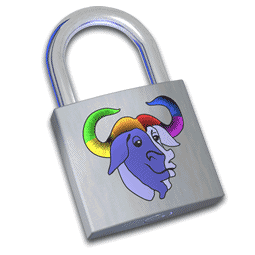
\includegraphics{images/gpg-logo.png}
%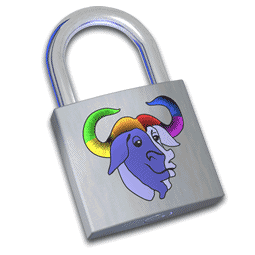
\includegraphics[scale=1]{images/gpg-logo.png}
\thispagestyle{empty}

%%\LARGE

%%\tableofcontents

\section{What is GPG?}

\textbf{GPG}, or The GNU Privacy Guard is, in a nutshell, a free and easy way to securely send and receive emails. The way most emails are currently sent is completely insecure, and is directly analogous to sending all of your mail on a postcard, available for any postman or eavesdropper along the way to read: we don't think this is good enough, and want to encourage more people to care about their privacy.\\
\textbf{GPG} allows you to send \textbf{completely secure} emails to anyone else with an email address and a key.

\section{Requirements}

Using the \Lclass{leaflet} class requires that the final
document is created in PostScript or PDF format, using
\begin{itemize}
  \item \TeX{} and \Lprog{dvips}, or
  \item pdf\TeX{}, or
  \item V\TeX{} in PS or PDF mode.
\end{itemize}
(Some other drivers supported by standard \LaTeX{} work as well.)

The non-standard macro package \Lpack{everyshi} \cite{cit:everyshi} is
used by the \Lclass{leaflet} class.
















\loggingall
\end{document}
\endinput
%%
%% End of file `leaflet-manual.tex'.
